\section{Durchführung}
\label{sec:Durchführung}

\begin{figure}
    \centering
    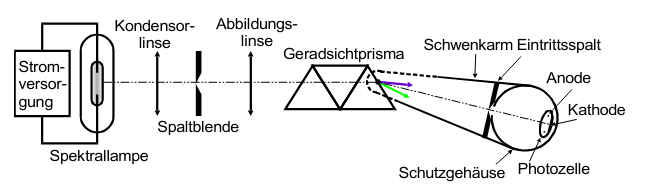
\includegraphics[width=0.7\textwidth]{aufbaru.png}
    \caption{Versuchsanordnung zur Untersuchung des Photoeffekts.}
    \label{fig:Versuchsanordnung}
\end{figure}

In Abbildung \ref{fig:Versuchsanordnung} ist der Versuchsaufbau gezeigt, der genutzt wird, um den Photoeffekt genauer zu betrachten. Hier wird als Strahlungsquelle eine 
Quecksilberlampe verwendet.\\
Aufgrund der hohen Empfindlichkeit der Messapparatur ist es wichtig, dass alles gut justiert ist. Das aus der Kondensorlinse kommende Licht soll so auf den Spalt treffen, 
dass die Breite der Spaltblende genau ausgefüllt ist. Dann können optimale Ergebnisse erzielt werden. \\
Durch Verschiebung der Abbildungslinse wird das Bild des vom Prisma zerlegten Lichtes so eingestellt, dass sich am Eingang der Photozelle scharfe Spektrallinien ergeben.\\
\\
\noindent Zunächst werden die grüne, violette und rote Spektrallinie so justiert, dass sie genau auf den Eingang der Photozelle treffen. Dazu wird der Teil der Versuchsanordnung
mit der Lampe verschoben.\\
Für jede dieser Spektrallinien wird dann der Photostrom für eine Spannung ab 2 $\si{\volt}$ gemessen, wobei die Spannung in Schritten von $0.25 \si{\volt}$ verringert wird, bis die Spannung 
unter 0 fällt. Ab diesem Punkt wird die Spannung in $0.2 \si{\volt}$-Schritten verringert, bis der Photostrom verschwindet.\\
Anschließend wird die gelbe auf den Eingang der Photozelle ausgerichtet und der resultierende Photostrom im Bereich von $20$ bis $-20 \si{\volt}$ unter verschiedenen Schrittweiten gemessen. Bei höheren
Spannungen wird in $2 \si{\volt}$ Schritten gemessen, im Bereich von 2 bis -2 $\si{\volt}$ wird die Schrittweite auf $0.25 \si{\volt}$ verringert, daraufhin wieder auf $5 \si{\volt}$ 
vergrößert.